\section{Discussions}

\textbf{Difference of applied scenes:}
All of our experiements are executed using Logitech C920 camera, which is a desktop camera for video calls so the range is used for a person sitting in front of a computer.
However, our potential use case is for phone taking photos.
Phone cameras obviously have larger range, especially a much further distance.

\textbf{Focus function:}
The current focus function is still very inefficient.
Nowadays cameras tend to only includes a few sampling pixels to calculate the derivative sum.
These samples usually are in the central area of the photos.
This way the calculation of focus functions are greatly speeded up.

\textbf{Minimum step of focus position:}
Currently all the experiments are done under Linux, where minimal step of 5mm is supported by UVC cameras under Linux.
If we move the experiments to Windows where 1mm is supported, that indicates 5 more captures on average for a single photo, which further extends the speedup effect of \sysname.

\textbf{Hardware time:}
The scripts and codes in this experiment produce ridiculously long focusing time, which lasts seconds.
This is caused by the software implementation.
In real cameras, all the steps mentioned are implemented in hardware, which should be hundreds of times faster.

\begin{figure}[tb!]
	\begin{center}
		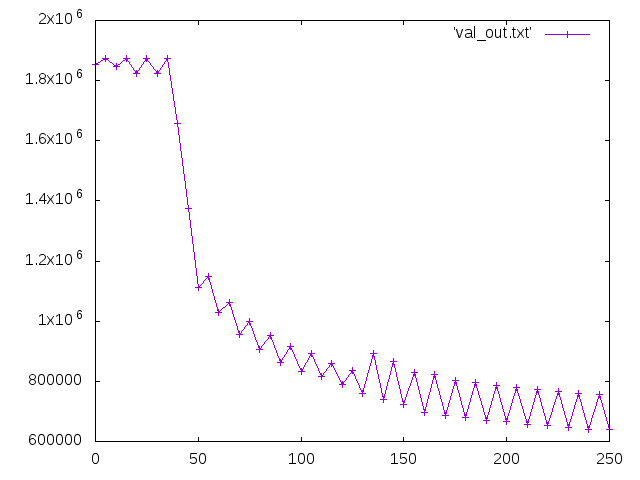
\includegraphics[width=2in]{outplot}
	\end{center}
	\caption{Wave effect caused by exposure time}
	\label{f:outplot}
\end{figure}

\textbf{Exposure, white balance play important parts:}
In Figure~\ref{f:outplot}, we present the function value results when we have auto exposure time enabled.
The photo is the same as human, and the function value is shown in Figure~\ref{f:humanplot}.
We can see that the general pattern is similar but the wave effect exists when auto exposure is enabled.
With auto exposure, the brightness and contrast of the figure is greatly impacted so we need to fix these third-party parameters to ensure stablized curve.
